\section{Inclusion--exclusion}
\emph{การเพิ่มเข้า--ตัดออก} (inclusion--exclusion) เป็นกฎการนับกฎหนึ่งที่ช่วยในการหาจำนวนสมาชิกของเซต รวมถึงจำนวนวิธีที่สามารถกระทำการต่างๆ ซึ่งการนับจำนวนดังกล่าวโดยตรงนั้นมีความซับซ้อน

% \newcommand\cnode[1]{\tikz{\node[draw,inner sep=2pt]{#1}}}
\newcommand\cnode[1]{\fbox{#1}}

\begin{example}
หากเซต $A$ มีสมาชิก $a$ ตัว และเซต $B$ มีสมาชิก $b$ ตัว แล้วทั้งสองเซตนี้มีสมาชิกรวมกันทั้งหมดกี่ตัว

หากทั้งสองเซตนี้ไม่มีสมาชิกร่วมกันเลย กล่าวคือ $A\cap B=\emptyset$ จะได้ว่า จำนวนสมาชิกคือ $a+b$ \enskip แต่ในกรณีทั่วไปนั้น ทั้งสองเซตนี้อาจจะมีสมาชิกร่วมกันได้ ดังรูป \enskip ดังนั้น การนับจำนวนสมาชิก จำเป็นต้องหักลบส่วนที่ทับซ้อนกันออกไป
\begin{center}
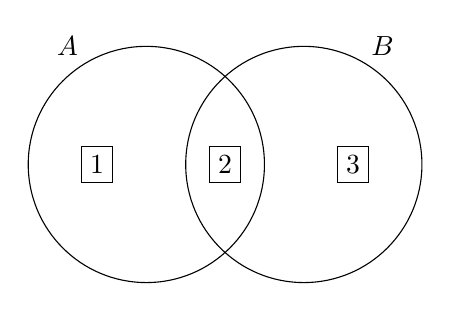
\begin{tikzpicture}
\draw (-1,0) circle (1.5);
\draw (1,0) circle (1.5);

\node at (-2,1.5) {$A$};
\node at (2,1.5) {$B$};

\node at (-1.625,0) {\cnode{1}};
\node at (0,0) {\cnode{2}};
\node at (1.625,0) {\cnode{3}};
\end{tikzpicture}
\end{center}

จากรูป จะเห็นว่า สมาชิกของเซต $A$ นั้นสามารถอยู่ได้ในบริเวณที่~\cnode{1} และ~\cnode{2} ส่วนสมาชิกของเซต $B$ นั้นสามารถอยู่ได้ในบริเวณที่~\cnode{2} และ~\cnode{3} กล่าวคือ $a=\cnode{1}+\cnode{2}$ และ $b=\cnode{2}+\cnode{3}$ \enskip ดังนั้น $|A|+|B|=a+b=\cnode{1}+\cnode{2}+\cnode{2}+\cnode{3}$ \enskip จะเห็นว่า บริเวณที่~\cnode{2} นั้นถูกนับซ้ำกันสองครั้ง นั่นคือ หากจะหาจำนวนสมาชิกของทั้งสองเซตรวมกันให้ถูกต้อง จะต้องหักลบบริเวณที่~\cnode{2} ออกไป ซึ่งบริเวณที่สองนี้คือ $A\cap B$ \enskip จึงสรุปได้ว่า $|A\cup B|=|A|+|B|-|A\cap B|$
\end{example}

\begin{example}
จำนวนสมาชิกของ $|A\cup B\cup C|$ สามารถคำนวณได้ดังนี้ \enskip ก่อนอื่น พิจารณาส่วนต่างๆ ของเซต $A$, $B$, และ $C$ ที่อาจจะทับซ้อนกัน ดังรูป
%
\begin{center}
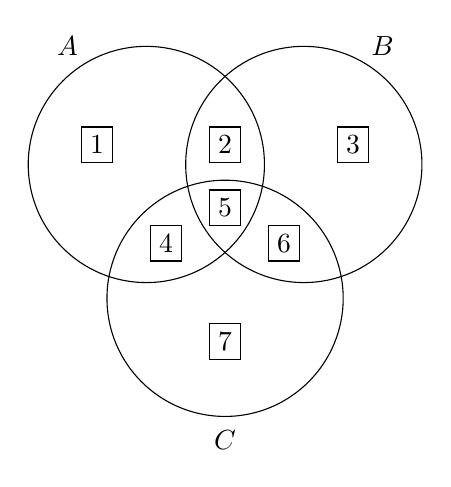
\begin{tikzpicture}
\draw (-1,0) circle (1.5);
\draw (1,0) circle (1.5);
\draw (0,-1.7) circle (1.5);

\node at (-2,1.5) {$A$};
\node at (2,1.5) {$B$};
\node at (0,-3.5) {$C$};

\node at (-1.625,0.25) {\cnode{1}};
\node at (0,0.25) {\cnode{2}};
\node at (1.625,0.25) {\cnode{3}};
\node at (-0.75,-1) {\cnode{4}};
\node at (0,-0.55) {\cnode{5}};
\node at (0.75,-1) {\cnode{6}};
\node at (0,-2.25) {\cnode{7}};
\end{tikzpicture}
\end{center}

จากรูป สมาชิกของเซตต่างๆ จะอยู่ในบริเวณต่อไปนี้
\begin{itemize}[]
\item เซต $A$ ประกอบไปด้วยบริเวณ $\cnode{1}+\cnode{2}+\cnode{4}+\cnode{5}$
\item เซต $B$ ประกอบไปด้วยบริเวณ $\cnode{2}+\cnode{3}+\cnode{5}+\cnode{6}$
\item เซต $C$ ประกอบไปด้วยบริเวณ $\cnode{4}+\cnode{5}+\cnode{6}+\cnode{7}$
\end{itemize}
ดังนั้น หากคำนวณ $|A|+|B|+|C|$ จะได้
\begin{align*}
|A|+|B|+|C|
&= \left(\cnode{1}+\cnode{2}+\cnode{4}+\cnode{5}\right) + \left(\cnode{2}+\cnode{3}+\cnode{5}+\cnode{6}\right) + \left(\cnode{4}+\cnode{5}+\cnode{6}+\cnode{7}\right) \\
&= \cnode{1}+\cnode{3}+\cnode{7}+2\cdot\cnode{2}+2\cdot\cnode{4}+2\cdot\cnode{6}+3\cdot\cnode{5}
\end{align*}
จะเห็นว่า บริเวณที่ \cnode{2}, \cnode{4}, \cnode{5}, และ \cnode{6} นั้นถูกนับซ้ำ จึงจำเป็นต้องหักการนับในบริเวณนี้ออก \enskip พื้นที่ในบริเวณดังกล่าวเป็น intersections ของสองเซต กล่าวคือ
\begin{itemize}[]
\item $A\cap B$ ประกอบไปด้วยบริเวณ $\cnode{2}+\cnode{5}$
\item $A\cap C$ ประกอบไปด้วยบริเวณ $\cnode{4}+\cnode{5}$
\item $B\cap C$ ประกอบไปด้วยบริเวณ $\cnode{5}+\cnode{6}$
\end{itemize}
ดังนั้น หากหักผลลัพธ์จากก่อนหน้านี้ด้วยบริเวณดังกล่าวออก จะได้
\begin{align*}
\lefteqn{|A|+|B|+|C|-|A\cap B|-|A\cap C|-|B\cap C|} \\
&= \cnode{1}+\cnode{3}+\cnode{7}+2\cdot\cnode{2}+2\cdot\cnode{4}+2\cdot\cnode{6}+3\cdot\cnode{5} - \left(\cnode{2}+\cnode{5}\right) - \left(\cnode{4}+\cnode{5}\right) - \left(\cnode{5}+\cnode{6}\right) \\
&= \cnode{1}+\cnode{3}+\cnode{7}+\cnode{2}+\cnode{4}+\cnode{6}
\end{align*}
อย่างไรก็ดี เมื่อทำการหักลบส่วนดังกล่าวออกไปแล้ว จะเห็นว่า บริเวณที่ \cnode{5} นั้นถูกหักลบออกมากเกินไป จึงจำเป็นต้องบวกจำนวนสมาชิกในบริเวณนี้เพิ่มกลับเข้ามา ซึ่งบริเวณนี้คือ $A\cap B\cap C$ นั่นเอง \enskip ดังนั้น จำนวนสมาชิกทั้งหมดของ $A$, $B$, และ $C$ รวมกันคือ
\[|A\cup B\cup C|=|A|+|B|+|C|-|A\cap B|-|A\cap C|-|B\cap C|+|A\cap B\cap C|\]
จะเห็นว่า เราใช้การเพิ่มเข้า--ตัดออก ในการนับจำนวนสมาชิกของเซต โดยบวกจำนวนสมาชิกในเซตเดี่ยวๆ เข้ามาก่อน จากนั้น หักลบด้วยจำนวนสมาชิกของผลลัพธ์จากการ intersect สองเซตเข้าด้วยกัน และในท้ายที่สุด เราบวกเพิ่มด้วยจำนวนสมาชิกจากการ intersect ทั้งสามเซตเข้าด้วยกัน
\end{example}

\begin{example}
สวนสาธารณะแห่งหนึ่งมีทางเดินโดยรอบ ดังรูป \enskip ทางเข้าสวนสาธารณะแห่งนี้อยู่ที่จุดมุมล่างซ้าย ส่วนทางออกของสวนสาธารณะนั้นอยู่ที่จุดมุมบนขวา
\begin{center}
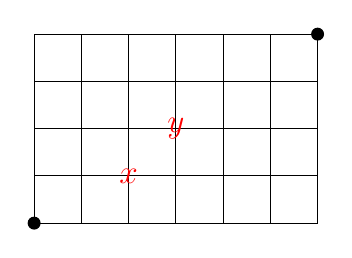
\begin{tikzpicture}[scale=0.6]
\draw (0,0) grid (6,4);
\draw[fill] (0,0) circle (0.125);
\draw[fill] (6,4) circle (0.125);
\node at (2,1) {\large\color{red} $x$};
\node at (3,2) {\large\color{red} $y$};
\end{tikzpicture}
\end{center}
เพื่อความสะดวกรวดเร็วและเป็นระเบียบในการเดินชมพรรณไม้ต่างๆ ในสวนสาธารณะ จึงมีกฎอยู่ว่า สามารถเดินตามเส้นไปทางขวา หรือเดินตามเส้นขึ้นด้านบนได้เท่านั้น \enskip หากต้องใช้กฎนี้ในการเดินสวนสาธารณะ จะมีวิธีการเดินจากจุดมุมล่างซ้ายไปยังจุดมุมบนขวาได้ทั้งหมดกี่วิธี

เนื่องจากเราไม่สามารถเดินไปทางซ้ายได้ และเราจำเป็นต้องเดินจากจุดซ้ายสุดไปยังจุดขวาสุด จะได้ว่า เราจำเป็นต้องเดินไปทางขวารวมแล้วทั้งหมด 6 ครั้งพอดี ไม่ขาดไม่เกิน \enskip ในทำนองเดียวกัน เนื่องจากเราไม่สามารถเดินลงได้ และเราจำเป็นต้องเดินจากจุดล่างสุดไปยังจุดบนสุด จะได้ว่า เราจำเป็นต้องเดินขึ้นรวมแล้วทั้งหมด 4 ครั้งพอดี ไม่ขาดไม่เกิน \enskip อย่างไรก็ดี ในการเดินแต่ละครั้ง เราสามารถเลือกได้ว่าจะเดินขวาหรือเดินขึ้น (หากเราไม่ได้อยู่ตำแหน่งขวาสุดหรือบนสุดของสวนสาธารณะแล้ว) \enskip กล่าวอีกนัยหนึ่ง ในทั้งหมด 10 ก้าวที่เราต้องเดินนั้น ต้องประกอบไปด้วยการเดินขวา 6 ก้าว และการเดินขึ้นอีก 4 ก้าว \enskip ดังนั้น จำนวนวิธีการเดินจากจุดล่างซ้ายไปยังจุดบนขวา ก็คือจำนวนวิธีการเลือกว่าจะเดินไปทางขวาในก้าวใดบ้าง \enskip เนื่องจากเราต้องเลือกเดินขวา 6 ก้าว จากทั้งหมด 10 ก้าว จะได้ว่า จำนวนวิธีเดินทั้งหมดที่เป็นไปได้คือ $\binom{10}{6}$

อย่างไรก็ดี เมื่อสวนสาธารณะเปิดทำการไปได้ระยะหนึ่ง ก็มีเสียงร่ำลือกันว่า จุด $x$ ในสวนสาธารณะ (ดังแสดงในรูป) เป็นจุดที่น่าสนใจจุดหนึ่งที่ควรเดินผ่าน \enskip หากต้องการเดินผ่านจุด $x$ ในสวนสาธารณะ จะมีวิธีเดินจากจุดล่างซ้ายไปยังจุดบนขวาได้ทั้งหมดกี่วิธี

เนื่องจากเราจำเป็นต้องเดินผ่านจุด $x$ แสดงว่า หากเราอยู่ทางด้านซ้ายของ $x$ แล้วเราจำเป็นจะต้องอยู่ด้านล่างของ $x$ ด้วย (มิฉะนั้น เราจะไม่สามารถเดินย้อนกลับมาที่จุด $x$ ได้อีก) \enskip ดังนั้น หากต้องการเดินผ่านจุด $x$ เราจำเป็นจะต้องเดินจากมุมล่างซ้ายให้ถึงภายใน 3 ก้าว โดยประกอบไปด้วยการเดินขวา 2 ก้าว และการเดินขึ้นอีก 1 ก้าว \enskip หากใช้วิธีการคิดเช่นเดียวกับสถานการณ์ก่อนหน้านี้ จะได้ว่า เราต้องเลือกว่าจะเดินไปทางขวาใน 2 ก้าวใดบ้างจากทั้งหมด 3 ก้าว ซึ่งสามารถทำได้ $\binom{3}{2}$ วิธี

จากนั้น เราต้องเดินจากจุด $x$ ไปยังจุดบนขวา ซึ่งประกอบไปด้วยการเดินขวา 4 ก้าว และการเดินขึ้น 3 ก้าว กล่าวคือ ในการก้าวทั้งหมด 7 ก้าวนั้น เราต้องเลือกที่จะเดินขวาทั้งหมด 4 ก้าว ซึ่งสามารถทำได้ $\binom{7}{4}$ วิธี

ดังนั้น การเดินจากจุดล่างซ้ายไปยังจุดบนขวาโดยผ่าน $x$ ประกอบด้วยสองขั้นตอนย่อยๆ ได้แก่ การเดินจากจุดล่างซ้ายไป $x$ และการเดินจาก $x$ ไปยังจุดบนขวา จึงสรุปได้ว่า จำนวนวิธีการเดินทั้งหมดในลักษณะดังกล่าวที่เป็นไปได้คือ $\binom{3}{2}\binom{7}{4}$ โดยใช้กฎการคูณ

ในทำนองเดียวกัน หากต้องการเดินจากจุดล่างซ้ายไปยังจุดบนขวา โดยต้องผ่านจุด $y$ (แต่ไม่จำเป็นต้องผ่านจุด $x$) จะสามารถทำได้ $\binom{5}{3}\binom{5}{3}$ วิธี

แต่หากต้องการเดินผ่านทั้งจุด $x$ และ $y$ ทั้งคู่ เราต้องเดินจากจุดล่างซ้ายไปยัง $x$ ก่อน แล้วเดินจาก $x$ ไป $y$ และเดินจาก $y$ ไปยังจุดบนขวาในท้ายที่สุด \enskip หากนำจำนวนวิธีที่ทำได้ในแต่ละขั้นตอนมาคูณกันโดยใช้กฎการคูณ จะได้ว่า จำนวนวิธีเดินให้ผ่านทั้ง $x$ และ $y$ คือ $\binom{3}{2}\binom{2}{1}\binom{5}{3}$

อนึ่ง เมื่อเวลาผ่านไป ผู้เยี่ยมชมสวนสาธารณะแห่งนี้ได้ให้ความสนใจกับจุด $x$ และ $y$ มากขึ้นจนทำให้สองจุดนี้เกิดความแออัด \enskip นักท่องเที่ยวบางส่วนจึงตัดสินใจที่จะไม่เดินผ่าน $x$ หรือ $y$ เลย (กล่าวคือ ไม่ผ่าน $x$ และไม่ผ่าน $y$) \enskip นักท่องเที่ยวเหล่านี้จะมีวิธีเดินที่เป็นไปได้ทั้งหมดเท่าใด

วิธีการคำนวณวิธีหนึ่งที่ทำได้ คือการนำจำนวนวิธีเดินทั้งหมดจากจุดล่างซ้ายไปจุดบนขวา หักลบด้วยจำนวนวิธีเดินที่ผ่าน $x$ และหักลบด้วยจำนวนวิธีเดินที่ผ่าน $y$ 
\enskip อย่างไรก็ดี จะเห็นว่า วิธีเดินที่ผ่านทั้ง $x$ และ $y$ นั้นจะถูกหักลบไปถึงสองครั้ง เนื่องจากวิธีที่เดินผ่าน $x$ ที่เราหักออกไปนั้นอาจจะผ่าน $y$ ด้วย และวิธีที่เดินผ่าน $y$ ที่เราหักออกไปนั้นอาจจะผ่าน $x$ ด้วย \enskip หากจะนับจำนวนวิธีให้ถูกต้อง เราต้องบวกเพิ่มด้วยจำนวนวิธีเดินที่ผ่านทั้ง $x$ และ $y$ กลับเข้าไปใหม่ \enskip ดังนั้น หลักการ inclusion--exclusion จึงทำให้เราคำนวณวิธีการเดินทั้งหมดที่เป็นไปได้โดยไม่ผ่าน $x$ หรือ $y$ เลย ซึ่งก็คือ
\[\binom{10}{6}-\binom{3}{2}\binom{7}{4}-\binom{5}{3}\binom{5}{3}+\binom{3}{2}\binom{2}{1}\binom{5}{3}\]
\end{example}

\begin{example}
มีซาลาเปา 5 ไส้ ไส้ละ 10 ลูกวางจำหน่ายอยู่ \enskip ต้องการซื้อซาลาเปารวม 41 ลูก โดยต้องซื้อไส้ละอย่างน้อย 1 ลูก จะสามารถทำได้กี่วิธี

แรกเริ่ม หากเราซื้อซาลาเปา 41 ลูก ไส้ละอย่างน้อย 1 ลูก (โดยแต่ละไส้จะซื้อกี่ลูกก็ได้) จะสามารถทำได้ $\binom{40}{4}$ วิธี จากกฎ stars and bars

แต่จะเห็นว่า บางวิธีข้างต้นนั้นใช้การไม่ได้ เนื่องจากอาจจะมีบางไส้ที่เราตัดสินใจซื้อมาเกิน 10 ลูก ซึ่งจำนวนซาลาเปาที่วางจำหน่ายนั้นมีไม่เพียงพอต่อความต้องการ \enskip เราจึงต้องหักลบวิธีเหล่านี้ออกไปจากจำนวนวิธีข้างต้น \enskip ตัวอย่างเช่น เราจำเป็นต้องหักลบวิธีที่เราจะซื้อซาลาเปาไส้แรกอย่างน้อย 11 ลูกออกไป เนื่องจากจำนวนซาลาเปาที่วางจำหน่ายนั้นมีไม่เพียงพอ ในกรณีนี้ จำนวนวิธีการซื้อซาลาเปาไส้แรกอย่างน้อย 11 ลูก (ส่วนไส้ที่เหลือนั้นซื้ออย่างน้อย 1 ลูก) จะเท่ากับจำนวนวิธีการซื้อซาลาเปารวม 31 ลูก ไส้ละอย่างน้อย 1 ลูก (จากนั้น ซื้อไส้แรกมาเพิ่มอีก 10 ลูก) ซึ่งสามารถทำได้ $\binom{30}{4}$ วิธี

จะเห็นว่า หากเปลี่ยนไส้แรกเป็นไส้อื่นๆ ที่จำนวนเกินกว่าที่วางจำหน่าย จะนับจำนวนวิธีได้เท่ากันเช่นกัน \enskip เนื่องจากไส้ที่เกินมาเป็นไปได้ทั้งหมด 5 ไส้ จะได้ว่า จำนวนวิธีที่มีซาลาเปา 1 ไส้ไม่เพียงพอต่อความต้องการของเรา (และจำเป็นต้องหักออกไป) คือ $5\binom{30}{4}=\binom{5}{1}\binom{30}{4}$ \enskip กล่าวอีกนัยหนึ่ง เราสามารถเลือกไส้ที่จะเกินมาจาก 5 ไส้ได้ $\binom{5}{1}$ แบบ และในแต่ละแบบนั้น จำนวนวิธีที่สามารถซื้อซาลาเปาไส้นั้นๆ เกินมาได้คือ $\binom{30}{4}$

อย่างไรก็ดี เมื่อเราหักลบจำนวนวิธีดังข้างต้นออกไป วิธีการซื้อที่มีซาลาเปา 2 ไส้เกินกว่าที่วางจำหน่ายนั้นได้ถูกหักลบออกไปซ้ำซ้อน \enskip ตัวอย่างเช่น วิธีที่มีซาลาเปาทั้งไส้ที่ 1 และ 2 เกินกว่าจำนวนที่วางจำหน่ายทั้งคู่ จะถูกหักลบไปหนึ่งครั้งเมื่อเราพิจารณาจำนวนวิธีที่ซื้อไส้ที่ 1 เกิน 10 ลูก และอีกครั้งหนึ่งเมื่อเราพิจารณาจำนวนวิธีที่ซื้อไส้ที่ 2 เกิน 10 ลูก \enskip ดังนั้น เราจึงต้องบวกจำนวนวิธีที่มีซาลาเปา 2 ไส้เกินกว่าที่มีจำหน่ายทดกลับเข้าไป \enskip ก่อนอื่น ต้องเลือกว่าสองไส้ใดจะเป็นไส้ที่ต้องการพิจารณา ซึ่งเป็นไปได้ $\binom{5}{2}$ แบบ \enskip จากนั้น ในแต่ละแบบ ต้องคำนวณวิธีที่ซาลาเปาสองไส้นี้มีจำนวนมากกว่าที่วางจำหน่าย กล่าวคือ ต้องซื้อสองไส้นี้ไส้ละอย่างน้อย 11 ลูกทั้งคู่ \enskip จำนวนวิธีดังกล่าวเทียบเท่ากับการซื้อซาลาเปาสองไส้นี้มาไส้ละ 10 ลูกก่อน จากนั้น ซื้อซาลาเปาอีกรวม 21 ลูก ไส้ละอย่างน้อย 1 ลูก ซึ่งสามารถทำได้ $\binom{20}{4}$ วิธี \enskip จึงสรุปได้ว่า จำนวนวิธีทั้งหมดที่เราต้องทดกลับเข้าไปคือ $\binom{5}{2}\binom{20}{4}$

เมื่อเราทดจำนวนวิธีข้างต้นกลับเข้าไปแล้ว จะสังเกตได้ว่า เราได้ทดจำนวนวิธีที่มีซาลาเปา 3 ไส้เกินกว่าที่วางจำหน่ายเข้าไปซ้ำซ้อนในลักษณะเดียวกันกับก่อนหน้านี้ \enskip เราจึงต้องหักจำนวนวิธีที่มีซาลาเปา 3 ไส้เกินกว่าที่มีจำหน่ายออกไป \enskip ก่อนอื่น ต้องเลือกว่า 3 ไส้ใดจะมีจำนวนลูกเกินกว่าที่วางจำหน่าย ซึ่งเลือกได้ $\binom{5}{3}$ แบบ ในแต่ละแบบ ต้องซื้อ 3 ไส้นี้ไส้ละอย่างน้อย 11 ลูก \enskip หากซื้อ 3 ไส้นี้ไส้ละ 10 ลูกก่อน จะเหลือซาลาเปาที่ยังต้องซื้ออีก 11 ลูก ไส้ละอย่างน้อย 1 ลูก ซึ่งสามารถทำได้ $\binom{10}{4}$ วิธี \enskip จึงสรุปได้ว่า จำนวนวิธีทั้งหมดที่เราต้องหักออกไปคือ $\binom{5}{3}\binom{10}{4}$

ณ จุดนี้ เราสามารถตั้งข้อสังเกตได้ว่า เมื่อใดก็ตามที่เราหักจำนวนวิธีที่เราไม่ต้องการออก จะมีบางวิธีที่ถูกหักออกซ้ำซ้อน และในทางกลับกัน เมื่อใดก็ตามที่เราทดจำนวนวิธีที่เราหักออกมามากเกินไปกลับเข้าไป ก็จะมีบางวิธีที่ถูกทดกลับเข้าไปซ้ำซ้อนอีกเช่นกัน จึงทำให้เราจำเป็นต้องสลับการเพิ่มเข้า--ตัดออกดังข้างต้น \enskip ในท้ายที่สุดนี้ หากใช้เหตุผลในลักษณะเดียวกันกับข้างต้น จะได้ว่า เราต้องทดจำนวนวิธีที่มีซาลาเปา 4 ไส้เกินกว่าที่วางจำหน่ายกลับเข้าไปใหม่ \enskip อย่างไรก็ดี หากมีซาลาเปา 4 ไส้ที่ความต้องการซื้อของเรานั้นเกินกว่าที่มีวางจำหน่าย จะเห็นว่า เราต้องซื้อซาลาเปาไส้เหล่านี้ไส้ละอย่างน้อย 11 ลูก ซึ่งแปลว่าเราจะต้องซื้อซาลาเปาไปแล้วอย่างน้อย 44 ลูก เกินกว่าจำนวนที่กำหนดไว้ \enskip ดังนั้น จำนวนวิธีการซื้อซาลาเปา 41 ลูก โดยที่มี 4 ไส้ที่ซื้อเกินไส้ละ 10 ลูก นั้นเป็น 0 จึงไม่มีวิธีใดๆ ให้ทดกลับเข้าไปอีก และทำให้กระบวนการเพิ่มเข้า--ตัดออกนั้นสิ้นสุดลง

จึงสรุปได้ว่า จำนวนวิธีซื้อซาลาเปาทั้งหมดที่เป็นไปได้ คือ
\[\binom{40}{4}-\binom{5}{1}\binom{30}{4}+\binom{5}{2}\binom{20}{4}-\binom{5}{3}\binom{10}{4}\]
\end{example}
